\documentclass[12pt]{article}

\usepackage{fancyhdr}
\usepackage{geometry}
\usepackage{ucs}
\usepackage[utf8x]{inputenc}
\usepackage[T1]{fontenc}
\usepackage[ngerman]{babel}
\usepackage{amsmath,amssymb,amstext}
\usepackage{hyperref}
\usepackage{cancel}
\usepackage{dsfont}
\usepackage{mathrsfs}
\usepackage{physics}
\usepackage{lmodern}
\usepackage{enumerate}
\usepackage{enumitem}
\usepackage{graphicx}
\usepackage{listings, color}
\usepackage[labelfont=bf]{caption}
\usepackage{titling}

\lstset{basicstyle=\scriptsize} %Quellcode mit Umlauten und ganz klein
\lstset{literate=
  {Ö}{{\"O}}1
  {Ä}{{\"A}}1
  {Ü}{{\"U}}1
  {ß}{{\ss}}2
  {ü}{{\"u}}1
  {ä}{{\"a}}1
  {ö}{{\"o}}1
}


%Geometrie----------------------------------------------------------------------------------------------------------

\geometry{a4paper, top=25mm, left=15mm, right=15mm, bottom=25mm,headsep=10mm, footskip=10mm}
\pagestyle{fancy}
\setlength{\parindent}{0pt} %Zeileneinrückung

\fancyhf{} %Setzt voreingestellte Kopf-und Fußzeilen-Eigenschaften zurück

\lhead{\nouppercase{\leftmark}}
\chead{}
\rhead{\thepage}

\lfoot{}
\cfoot{}
\rfoot{}

\title{\vspace{0cm}{\Huge Fortgeschrittenen-Praktikum I:\\ \vspace{1cm} Ultraschall}}
\author{Saskia Bondza\\Simon Stephan}
\date{durchgeführt am 20./21.09.2016}

\pretitle{%
  \begin{center}
  \LARGE
  
\includegraphics[width=6cm,]{figures/siegel}\\[\bigskipamount]
}
\posttitle{\end{center}}

%neue Commands----------------------------------------------------------------------------------------------------------
\newcommand{\nab}{\vec{\nabla}} %direkter Befehl mit Vektorpfeil
\newcommand{\gra}[3][0.7]{
	\begin{minipage}[h!]{\textwidth}
		\centering
		\includegraphics[width=#1\textwidth]{figures/#2.png}
		\captionof{figure}{#3}
	\end{minipage}
	\vskip 30 pt
}
\newcommand{\graTwo}[4][0.5]{
	\begin{minipage}[h!]{\textwidth}
		\centering
		\includegraphics[width=#1\textwidth]{figures/#2.png}
		\includegraphics[width=#1\textwidth]{figures/#3.png}
		\captionof{figure}{#4}
	\end{minipage}
	\vskip 30 pt
}
\newcommand{\del}[2][]{\frac{\partial #1}{\partial #2}}
\newcommand{\code}[1]{\texttt{#1}}
\DeclareMathOperator{\sinc}{\mathit{sinc}}
\DeclareMathOperator{\rect}{\mathit{rect}}
\DeclareMathOperator{\comb}{\mathit{comb}}

%Titel,Inhalt----------------------------------------------------------------------------------------------------------

\begin{document}
\pagenumbering{gobble} %verstecke Seitenzahl
\maketitle
\newpage

\thispagestyle{empty}
\section*{Abstract}


In diesem Versuch wird über die Messung von Beugungs-Spektren eines He-Ne-Lasers ($\lambda = 632,8nm$) die Gitterkonstante verschiedener Gitter (Sinusgitter, Amplitudengitter) und die Aperturfunktion eines bestimmten Gitters bestimmt. Der Hauptteil des Versuches beschäftigt sich mit der Untersuchung von Ultraschallwellen in Flüssigkeit als Phasengitter. Dazu wird die Intensitätsänderung der Beugungsordnung in Abhängigkeit der Spannung des Schallerzeugers (Piezoquarz) ausgewertet, die Wellenlänge der Ultraschallwelle bestimmt und mit der Raman-Nath-Theorie verglichen.

\newpage
\tableofcontents
\newpage

%Schreiben----------------------------------------------------------------------------------------------------------
\pagenumbering{arabic} %verstecke Seitenzahl
\section{Einleitung}





\newpage
\section{Theoretische Grundlagen}

\subsection{Beugung}

Trifft eine Lichtwelle auf ein Hindernis z.B. einen Spalt wird das Phänomen der Beugung beobachtet. In Abbildung \ref{Fraunhofer} ist  der Grundaufbau eines Experiments zum Nachweis von Beugungsphänomenen (Fraunhofersche Anordnung) dargestellt, der in diesem Experiment verwendet wird. 

\gra{Fraunhofer}{Fraunhofersche Anordnung \label{Fraunhofer}}   

Ein paralleles Lichtbündel lässt sich durch eine Sammellinse, die im Abstand einer Brennweite zur Lichtquelle steht, erzeugen. Am Gitter wird das Licht dann gebeugt. Dabei gilt das Huygen'sche Prinzip, nach dem jeder Punkt einer Wellenfront Quelle einer Kugelwelle mit gleicher Frequenz der ursprünglichen Welle ist. Die Amplitude des optischen Feldes hinter dem Gitter ergibt sich demnach aus der Überlagerung aller so entstehenden Wellen unter Berücksichtigung ihrer Amplitude und Phase. Konstruktive und destruktive Interferenz (je nach Gangunterschied), die sich aus diesen Überlagerungen ergibt, bildet schließlich das charakteristische Beugungsmuster. Eine zweite Sammellinse bildet das Beugungsmuster auf einen Schirm ab, der als unendlich weit entfernt angenommen wird, sodass von Fraunhofer-Beugung gesprochen werden kann. Man spricht von Fraunhofer-Beugung, wenn das Beugungsmuster im Fernfeld beobachtet wird. Die Position der Maxima und Minima kann dann an Hand von geometrischen Überlegungen bestimmt werden oder alternativ mit Hilfe des Kirchhoff'schen Integraltheorems und den daraus abgeleiteten Fresnel-Kirchhoff-Integralformel (siehe \label{Fourier})

\subsection{Fourieroptik}  

Aus dem  Kirchhoff'schen Integraltheorems lässt sich die Fresnel-Kirchhoff-Integralformel entwickeln, mit der sich die Beugung von Licht durch ein beliebiges Hindernis errechnen lässt. Die Geometrie des Hindernisses ist dabei durch die Aperturfunktion $g$ gegeben. Es gilt dann für die Intensitätsvertilung $I$ auf dem Schirm im Fernfeld: 

\begin{align}
I=|U(x_0)|^2=\left| \int\limits_{-\infty}^{\infty} g(x,y)e^{-ikx}dx \right|^2
\end{align}



Die Intensitätsverteilung auf dem Schirm ist also das Betragsquadrat der Fouriertransformierten. Umgekehrt lässt sich damit auch die Aperturfunktion aus einer beobachteten Intensitätsverteilung berechnen. Im folgenden werden wir die Aperturfunktion ud die Intenstitätsverteilung für einen Einzelspalt und ein Gitter genauer betrachten.

\subsection{Einzelspalt}
       
Die Aperturfunktion eines Einzelspaltes mit der Breite $b$ un der Länge $l$ ist wie folgt gegeben:

\begin{align}
g(x)=\begin{cases}1 &\mbox{ falls }|x|\leq\frac{b}{2}\\0 &\mbox{ sonst }\end{cases}
\end{align}

Die Fouriertransformation dieser ist durch die $sinc$ Funkion gegeben:

\begin{align}
\mathscr{F}\left[ g(x) \right] = \left| b\right| \cdot \sinc\left( \frac{k \cdot b}{2}\right)  = 2 \cdot \left| b\right| \cdot \frac{\sinc\left( \frac{k \cdot b}{2}\right)}{k \cdot b}
\end{align}

\gra{Einzelspalt}{Fourierpaar für einen Einzelspalt}

Die Intensitätsverteilung des Beugungsmusters im Fernfeld ist somit:

\begin{align}
I = \left| \mathscr{F}\left[ g(x) \right]\right| ^2 = \left( \left| b\right| \cdot \sinc\left( \frac{k \cdot \left| b\right| }{2} \right) \right) ^2
\end{align}

\subsection{Gitter mit N Linien}

Für ein Gitter der  Breite L mit N Linien, der Spaltbreite b und der Gitterkonstane K ergibt sich die Aperturfunktion durch Wiederholung der Funktion eines Einzelspaltes:

\begin{align}
g\left( x\right) = \left( \rect\left( \frac{x}{b}\right) * \comb \left( \frac{x}{K}\right) \right) \cdot \rect \left( \frac{x}{L}\right) 
\end{align}

wobei * eine Konvolution markiert und die Funktion $\comb$ wie folgt definiert ist:

\begin{align}
\comb\left(  \frac{x}{b}\right)  = \sum_{n = -\infty}^{+ \infty} \delta\left(x-n\cdot b \right) 
\end{align}

Die Fouriertransformierte der Aperturfunktion ist gegeben durch:

FORMEL!!!!!!!

\gra{bla}{Fraunhoferbeugungsmuster eines Gitters \cite{Demtröder}} 

Die Intensitätsverteilung des Lichts ergibt sich dabei als proportional zu folgendem Ausdrck:

\begin{align}
I(\Theta) &= \left| \mathscr{F}\left[ g(x) \right]\right| ^2 = \left(\frac{\sin\left(\beta (\Theta) \right) }{\beta(\Theta)} \right)^2 \cdot \left(\frac{\sin\left(N \gamma \right) }{N \sin (\gamma)} \right)^2\\
\beta(\Theta) &= \frac{kb\sin(\Theta)}{2}\\
\gamma(\Theta) &= \frac{kK\sin(\Theta)}{2}\\
\end{align}

Das Begungsmuster wird mit höheren Werten von N schmäler und die sekundären Maxima kleiner. Der Zusammenhang zwischen Beugungswinkel und Maxima m-ter Ordnung ist:

\begin{align}
m\lambda = Ksin(\Theta)
\end{align}

Der Beugungswinkel lässt sich aus dem Versuchsaufbau wie folgt berechnen:

\begin{align}
\Theta = \mathit{arctan}\left( \frac{x}{d}\right) 
\end{align}

wobei hier $x$ der Abstand zum Beugunsmaximum 0. Ordnung ist und $d$ der Abstand zwischen Schirm und Gitter.\\

Die Auflösung $a$ eines optischen Gitters ist definiert als: 

\begin{align}
a = \frac{\lambda}{\Delta \lambda}
\end{align}

dabei gibt $\lambda$ die Wellenlänge des Lichts und $\Delta \lambda$ den Wellenlängenabstand an, bei welchem eine andere Wellenlänge von $\lambda$ bei der Beugung noch unterscheidbar ist. REF
Das Auflösungsvermögen lässt sich außerdem auch wie folgt ausdrücken:
\begin{align}
a = N \cdot m
\end{align}

wobei $N$ die Anzahl der beleuchteten Spalte ist und $m$ die Anzahl beobachteter Maxima.

Die Aperturfunktion lässt sich aus der Fouriertransformierten der Intensitätsverteilung berechnen, indem man sie als Fourierreihe nähert, deren Koeffizienten den Wurzeln der Intensitäten der Maxima entsprechen:

\begin{align}
g(x) = \sum_{j = 0}^{\infty} \pm \sqrt{I_j}\cos\left( \frac{2 \pi j x}{K}\right) \label{Fourier1}
\end{align} 

In allen praktischen Anwendungen ist diese Summe endlich, da die Intensitäten der Maxima mit steigender Beugungsordnung zunehmend abnehmen. 

\subsection{Sinusgitter}

Die Aperturfunktion für ein Sinusgitter ist gegeben durch:

\begin{align}
g\left( x\right) &= \left[ \frac{1}{2} + \frac{m}{2} \cdot \cos\left( 2 \pi k_0 x \right)   \right] \cdot \rect \left( \frac{x}{b} \right)  &&\text{wobei } 0 < m < 1
\end{align}

wobei: 

\begin{itemize}
\item $m =$ Stärke der Modulation
\item $b =$ Begrenzung der Gitterstruktur
\item $k_0 = $ räumliche Frequenz
\end{itemize}

Die Intensitätsverteilung für ein Sinusgitter ist dementsprechend:

\begin{align}
I = \left| \mathscr{F}\left[ g(x) \right]\right| ^2 = \sinc^2 \left(bk \right) + \frac{m^2}{4}\cdot\sinc\left[  b \left( k + k_0\right) \right] + \frac{m^2}{4}\cdot\sinc\left[  b \left( k - k_0\right) \right]
\end{align}

\gra{Sinusgitter}{Fraunhoferbeugungsmuster für ein dünnes Sinusgitter \label{Sinusgitter}}

Aus Abbildung \ref{Sinusgitter} ist ersichtlich, dass es drei Hauptmaxima an den Stellen $k = 0$ 
sowie $ k = \pm 2 \pi z $ ( wobei $z$ die Entfernung zum Sinusgitter ist). Die Intensitäten der Maxima 1. Ordnung entsprechen dabei einem Viertel der Intensität des Maximums 0. Ordnung. Die Aperturfunktion kann mit ref!!!!!!! wie folgt ausgedrückt werden:

\begin{align}
g\left( x\right) = \sqrt{I_0} + \sqrt{I_1}\cdot\cos\left( \frac{2 \pi x}{K}\right) 
\end{align}


\subsection{Phasengitter}

Während Amplitudegitter lediglich die Amplitude gebeugten Lichtes modulieren, beeinflussen optische Gitter die Phase des durchlaufenden Lichts durch Variationen im Brechungsindex, während kein Intensitätsverlust statt findet. In Abbildung \ref{Phasengitter} ist das Fraunhoferbeugungsmuster eines Sinus-Phasengitters dargestellt.

\gra{Phasengitter}{Fraunhoferbeugungsmuster für ein Sinus - Phasengitter \label{Phasengitter}}

Die Aperturfunktion eines solchen Gitters ist wie folgt gegeben:

\begin{align}
g\left( x\right) = \exp^{i\frac{m}{2}\sin\left( 2 \pi k_0 x\right)} \cdot \rect\left( \frac{x}{b} \right) 
\end{align}

Die Fouriertransformation dieser Funktion lässt sich mit Hilfe der Besselfunktionen wie folgt angeben:

\begin{align}
\mathscr{F}\left[ g(x) \right] = \sum_{q = - \infty}^{+ \infty} J_q \frac{m}{2} b \cdot \sinc\left(b \left( k -q \cdot k_0\right) \right) 
\end{align}

Die Intensität der Hauptmaxima eines solchen Phasengitters ergibt sich zu:

\begin{align} \label{23}
I_q \left(k \right) = J_q ^2\frac{m}{2}
\end{align}
\subsection{Ultraschallphasengitter und Raman-Nath-Theorie}
\label{Raman-Nath}

Eine laufende Schallwelle verursacht periodische Dichteschwankungen in einem Medium, was wiederum periodische Schwankungen des Brechungsindexes zur Folge hat. Trifft ein kohärenter, paralleler Lichtstrahl (in diesem Experiment ein Heliu-Neon-Laser) nun senkrecht zur Ultraschallwelle auf das Medium, tritt das Licht phasenversetzt aus und im Fernfeld führt diese verzerrte Phasenfront zu einer Überlagerung und einem Beugungsbild. Der Brechungsindex $n$ eines schalldurchsetzten Mediums mit Schall der Wellenlänge $\Gamma$ ist gegeben durch:

\begin{align}
n\left(x \right) = n_0 + \Delta n \cdot \sin \left(\frac{2 \pi x}{\Gamma} \right) 
\end{align}
Die Intenität des Schalls $S$ ist proportional zum Quadrat der an der Ultraschallzelle angelegten Spannung $ U$. Dies bedeutet, dass duch anlegen verschiedener Spannungen die Dichte $\rho$ und damit der Brechungsindex varriert werden können:

\begin{align}
U^2 \propto S \propto \left( \frac{\Delta n}{n -1} \right)^2 = \left( \frac{\Delta \rho}{\rho_0}\right)^2  
\end{align}

Vorrasugesetzt die breite $D$ des schalldurchsetzten Mediums und die Schallintensität sind nicht zu hoch, lässt sich Gleichung \ref{23} mit der Raman-Nath-Theorie modifizieren. Die Variablen transformieren sich wie folgt:

\begin{align}
q &\rightarrow m\\
m &= \frac{\Delta n D 4 \pi}{\lambda}
\end{align}

Die Winkel, unter denen die Peaks des Beugungsmusters beobachtet werden, können wie folgt bestimmt werden:

\begin{align}
\sin\left( \Theta\right) = \pm m \frac{\lambda}{\Lambda}
\end{align}

Gleichung \ref{23} wird außerdem zu:

\begin{align}
I_m = J_m^2 \left( \frac{\Delta n D 2 \pi}{\lambda} \right) = J_m^2\left(\alpha U \right) 
\end{align}
\newpage
\section{Genereller Versuchsaufbau} \label{Aufbau}

\gra[1]{Versuchsaufbau}{Versuchsaufbau \label{Versuchsaufbau}}

In Abbildung \ref{Versuchsaufbau} ist der generelle Versuchsaufbau dargestellt, der in den eintelnen Versuchsteilen angepasst wird.
Der Laserstrahl eines Helium-Neon-Lasers mit der Wellenlänge $\lambda = 632.8 nm$ wird nach Aufteilen durch einen Strahlteiler  teilweise durch eine erste Sammellinse (Linse 1) aufgeweitet und beim Treffen auf eine zweite Sammellinse (Linse 2), welche im Abstand der Summe der beiden Brennweiten steht, parallelisiert. Das Lichtbündel wird dann nach Durchlauf durch eine Blende an einem Gitter (je nach Versuchsaufbau Sinus-, Amplituden-, oder Phasengitter) gebeugt und trifft auf einen rotierenden Spiegel. Auf Grund der Drehung wird das Beugungsmuster 12.5 mal pro Sekunde auf die Photodiode (Diode 2) projiziert. Das detektierte Signal wird verstärkt und an einem Oszilloskop, das mit einem Computer verbunden ist analysiert. Das Oszilloskop wird durch das Signal der ersten Photodiode getriggert, die das Signal des ungebeugten Lichtstrahls, das nach dem Strahlteiler direkt auf den rotierenden Spiegel trifft, detektiert.

\newpage

\section{Sinusgitter}

\newpage
\subsection{Versuchsaufbau und -Durchführung}

In diesem Teil des Versuchs wird ein vereinfachter Versuchsaufbau benutzt. Ein Laserstrahl trifft direkt auf das Sinusgitter und das Beugungsmuster ist auf einem Schirm wenige Zentimeter hinter dem Sinusgitter zu beobachten. Für fünf verschiedene Abstände zwischen Gitter und Schirm wird jeweils die Lage der Beugungsmaxima 1. Ordnung gemessen und hieraus die Gitterkonstante bestimmt, sodass wir über die Mittelung mehrerer Werte einen genaueren Wert für die Gitterkonstante des Sinusgitters erwarten.



\newpage
\subsection{Auswertung}

Aus den gemessenen Koordinaten der Punkte $P(x/y)$ der Maxima (siehe \ref{Laborheft})berechnen wir zunächst die Abstände $l_1 = \sqrt{x_1²+y_1²}$ und $l_2= \sqrt{x_2^2+y_2^2} $ zwischen dem Maximum $0.$ Ordnung und den Maxima $1.$ Ordnung. Aus den beiden Abständen zum linken und rechten Maximum $1.$ Ordnung berechnen wir einen gemittelten Abstand $l_{ges}$. Die Fehler berechnen wir mit Gauß'scher Fehlerfortpflanzung aus dem Fehler $s_{x/y}$ auf die Koordinaten:

\begin{align*}
s_{l_1} = s_{l_2} &= \sqrt{\left(\del[l]{x}\cdot s_{x/y}\right)^2+\left(\del[l]{y}\cdot s_{x/y}\right)^2}\\
&= s_{x/y}\\
\  \\
s_{l_{ges}} &= s_{x/y}/\sqrt{2}
\end{align*}

Wir erhalten:

 \vskip 10 pt
 \begin{table}[h!]
 {\centering{}
\begin{tabular}{c||c|c|c}
 					& $l_1$/cm 	& $l_2$/cm & $l{ges}$/cm	\\ \hline\hline
Messung 1		& $3.9 \pm 0.1$ 	&  $3.9 \pm 0.1$    	&  $3.95 \pm 0.07$ \\ \hline 
Messung 2	&	 $1.9 \pm 0.1$ 	   	&  $1.8 \pm 0.1$  	&  $1.87 \pm 0.07$  \\ \hline
Messung 3      	&  $5.0 \pm 0.1$  	&  $4.9 \pm 0.1$  &  $5.00 \pm 0.07$  \\ \hline
Messung 4    & $2.8 \pm 0.1$ & $2.9 \pm 0.1$ &   $2.88 \pm 0.07$        \\ \hline                                           
Messung 5  & $5.6 \pm 0.1$  & $5.7 \pm 0.1$ & $5.61 \pm 0.07$
 \end{tabular}}
 \caption{Abstände der Beugungsmaxima}
\end{table}
\vskip 10 pt

Hieraus lässt sich nun mit ref!!!!!! die Gitterkonstante $K$ berechnen wobei sich der Fehler wieder mit Gauß'scher Fehlerfortpflanzung berechnen lässt:

\begin{align*}
s_K = \sqrt{\left(\del[K]{l}\cdot s_{l}\right)^2+\left(\del[K]{d}\cdot s_{d}\right)^2}
\end{align*}

Wir erhalten:

\begin{itemize}
\item Messung 1: $K = 996 \pm 16$ nm
\item Messung 2: $K = 1082 \pm 40$ nm
\item Messung 3: $K = 989 \pm 13$ nm
\item Messung 4: $K = 994 \pm 23$ nm
\item Messung 5: $K = 995 \pm 12$ nm
\end{itemize}

Als Endergebnis berechnen wir nun noch das gewichtete Mittel mit Fehler:

\begin{align*}
K_{ges} &=\frac{\sum\limits_i \frac{1}{\sigma_i²} \cdot K_i}{\sum\limits_i \frac{1}{\sigma_i²}}\\
s_{K_{ges}} &= \frac{1}{\sum\limits_i \frac{1}{\sigma_i²}}
\end{align*}

und erhalten:

\begin{align*}
K_{ges} = 996 \pm 7 nm
\end{align*}

\newpage
\subsection{Diskussion}

\newpage
\section{Amplitudengitter}

\newpage
\subsection{Versuchsaufbau und -Durchführung}

In diesem Teil des Versuchs wird der generelle Aufbau aus Abschnitt \ref{Aufbau} durch Einsetzen fünf verschiedener Amplitudengitter modifiziert. Für jedes dieser Gitter wird das Beugungsspektrum am Oszilloskop aufgezeichnet und daraus jeweils die Gitterkonstante und das Auflösungvermögen bestimmt. Für das Gitter, für das wir die größte Anzahl an Beugungsmaxima beobachten können, bestimmen wir außerdem aus der Intensität der Beugungsmaxima und der zuvor bestimmten Gitterkonstante  die Aperturfunktion. Aus dieser bestimmen wir zusätzlich die Spaltbreite und das Verhältnis derer zu Gitterkonstante.


\subsection{Auswertung}

\subsubsection{Referenzgitter}

\label{Happyisttoll}

Da das Oszilloskop eine Zeitdifferenz zwischen den Maxima angibt und keine Winkel, wird mit einem Referenzgitter mit bekannter Gitterkonstante zunächst eine Eichung des Winkel-Zeit-Verhältnisses durchgeführt und ein Umrechnungsfaktor bestimmt. Wir tragen hierfür die Zeit über die theoretische Lage der Maxima auf, die sich aus \[\sin\theta=\frac{n\lambda}{K_R}\] mit $K_R = 0.125 mm$ ergibt und führen einen linearen Fit durch.

\vskip 10 pt
 \begin{table}[h!]
 {\centering{}
\begin{tabular}{c||c|c}
 m & $\sin(\theta)$ & t/$10^{-4}$ \\ \hline\hline
 -2 &$-0.0101$&    $ -1.3427 \pm 0.0011 $  \\ \hline
 -1 &$-0.0051$& $ -0.6719 \pm 0.0005 $     \\ \hline
 0 &$0$&  $ 0\pm 0.0004$         \\ \hline
 1 &$0.0051$&   $ 0.6729 \pm 0.0005 $        \\ \hline
 2 &$0.0101$&     $ 1.3479 \pm 0.0012 $        \\ \hline

 \end{tabular}
 
 \caption{Abstände der Beugungsmaxima}}
\end{table}
\vskip 10 pt

\graTwo[0.49]{referenzgitter}{Zeiteichung}{Zeit-Winkel-Eichung\label{EINHORN}}

Aus der Steigung des Linearen Fits (siehe Abbildung \ref{EINHORN} ) lässt sich nun der Faktor für die Umrechnung von Zeit nach Winkeln bestimmen:

\begin{align*}
a &= (74.35\pm0.05)\,\frac1{\mathrm{s}}&
\text{mit } a = \frac{\sin(\theta))}{t}
\end{align*}

\subsubsection{Bestimmung verschiedener Gitterkonstanten}\label{amplitudengitterkonstante}
Wir haben für 5 verschiedenen unbekannte Amplitudengitter Interferenzmuster aufgenommen und bestimmen nun aus diesen die jeweilige Gitterkonstante. Die Zeitabhängigkeit der Interferenzmuster werden nun mithilfe des in \ref{Happyisttoll} berechneten Wertes in eine $\sin\theta$-Abhängigkeit umgerechnet. Anschließend wird aus den Beugungsordnungen in Abhängigkeit der Positionen der Maxima die Gitterkonstante des jeweiligen Gitters bestimmt. Die Steigung $a$ des linearen Fits $m=\frac{K}{\lambda}\sin\theta$ beträgt nun $a=\frac{K}{\lambda}$. Damit gilt für die Gitterkonstante: $$K=a\cdot\lambda$$.

Wir erhalten nun mit dieser Rechnung die folgenden Werte für die Gitterkonstanten:
\begin{align*}
	K_1&=(129.26\pm0.07)\,\mathrm{\mu m}\\
	K_2&=(34.26\pm0.03)\,\mathrm{\mu m}\\
	K_3&=(102.9\pm0.3)\,\mathrm{\mu m}\\
	K_4&=(72\pm6)\,\mathrm{\mu m}\\
	K_5&=(51.57\pm0.08)\,\mathrm{\mu m}\\  \label{K1}
\end{align*}


\subsubsection{Aperturfunktion}


Wir bestimmen die Aperturfunktion für Gitter 1, da wir hier die meisten Maxima beobachten konnten (siehe Abbildung ref!!!).
Aus den Amplituden der gefitteten  Gaußfunktionen erhalten wir hierbei die Intensität, wobei wir wir für jedes Maximum die Amplitude aus linkem und rechtem Maximum gewichtet mitteln (siehe ref!!!). 
 \vskip 10 pt
 \begin{table}[h!]
 {\centering
\begin{tabular}{c||c|c|c}
 					& $I_1/V$ 	& $I_2/V$ & $I_{ges}/V$	\\ \hline\hline
Maximum 5. Ordnung     & $0.08 \pm 0.14$  & $0.040 \pm 0.009$      &  $0.04012 \pm  0.00008$                       \\ \hline
Maximum 4. Ordnung		& $0.186 \pm 0.009$ 	&  $0.177 \pm 0.009$    	&  $0.182 \pm 0.006$ \\ \hline 
Maximum 3. Ordnung	&	 $0.402 \pm 0.009$ 	   	&  $0.447 \pm 0.010$  	&  $0.425 \pm 0.007$  \\ \hline
Maximum 2. Ordnung    & $0.666 \pm 0.016$ & $0.681 \pm 0.014$ &   $0.6735 \pm 0.07$        \\ \hline                                           
Maximum 1. Ordnung      	&  $0.95 \pm 0.02$  	&  $0.92 \pm 0.02$  &  $0.935 \pm 0.014$  \\ \hline

Maximumg 0. Ordnung  & -  & - & $2.72 \pm 0.06$
 \end{tabular}
 \caption{Abstände der Beugungsmaxima}}
\end{table}
\vskip 10 pt


Aus diesen und der zuvor berechneten Gitterkonstante $K_1 = (129.26 \pm 0.07) \mu m$ (siehe \ref{K1} lässt sich mittels der Fourierreihe (siehe \ref{Fourier1}) nun die Aperturfunktion näherungsweise bestimmen:

\[g(x)\approx\sum^{5}_{k=0}\pm\sqrt{I_k}\cos\left(\frac{2k\pi x}{K_1} \right) \]

\gra{apertur}{Genäherte Aperturfunktion von Gitter 1 \label{kotz}} 



Aus der Aperturfunktion bestimmen wir nun die Spaltbreite $b$, indem wir das FHWM durch Bestimmung des Schnittpunktes der Aperturfunktion mit der Konstanten mit dem Wert $x=\frac{max}{2}$  berechnen (siehe Abbildung \ref{LONDOOON}), wobei max für das Maximum der Aperturfunktion steht.

\gra{Fehler-apertur}{Bestimmung der Spaltbreite aus der Aperturfunktion\label{LONDOOON}}

Den Fehler schätzen wir durch die Bestimmung des FHWM für eine "Ober- bzw. Untergrenze" der Aperturfunktion, d.h. für eine Aperturfunktion bei der die Fehler der Intensitäten addiert wurden (in blau) und eine Aperturfunktion bei der die Fehler der Intenstitäten subtrahiert wurden (in rot).

Wir erhalten:

\begin{itemize}
\item $FWHM = 11.31475 \mu m $
\item$ FWHM_{max} = 11.32025 \mu m  $
\item $ FWHM_{min} = 11.30991 \mu m  $
\end{itemize}

\begin{align*}
b = 2 \cdot FHWM = 22.630  \pm  0.010 \mu m
\end{align*}

wobei sich der Fehler wie folgt berechnet:

\begin{align*}
s_b = 2 \cdot s_{FWHM} = 2 \cdot \frac{FWHM_{max}-FWHM_{min}}{2} = 0.010 \mu m
\end{align*}

Das Verhältnis $V$ von Spaltbreite und Gitterkonstante ergibt sich zu:

\begin{align*}
V=\frac{b}{K_1} = 0.1751\pm 0.0008
\end{align*}
wobei der Fehler sich mit Gauß'scher Fehlerfortpflanzung berechnet: 
\begin{align*}
 s_V=V\sqrt{\left( \frac{s_b}{b}\right)^2 +\left( \frac{s_{K_1}}{K_1}\right)^2 }
\end{align*}


\newpage
\subsection{Diskussion\label{BOOOOOMMMM!!!!!!!!!}} 


\newpage
\section{Ultraschall-Phasengitter}


\subsection{Versuchsaufbau und -Durchführung}





\newpage
\subsection{Auswertung}
\subsubsection{Zeiteichung}
Wie in \ref{Happyisttoll} haben wir das Referenzgitter mit $K_R=125 \mu m$ zur Zeiteichung benutzt, indem wir die gemessene zeitliche Position der Beugungsmaxima mit der berechneten Position in folgende Beziehung gesetzt haben:
$$t=\frac1a\sin\theta$$

\graTwo[0.49]{ultraschall-eichgitter}{ultraschall-zeiteichung}{Interferenzmuster des Referenzgitters und linearer Fit zur Bestimmung des Umrechnungsfaktors\label{simonhatsverkackt}}

Aus dem linearen Fit der Zeit über den Sinus des Winkels (siehe Abbildung \ref{simonhatsverkackt}) erhalten wir:
\begin{align*}
a &=(70.64\pm0.06)\,\frac1{\mathrm{s}}&
\text{mit } a = \frac{\sin(\theta)}{t}
\end{align*}
Im restlichen Teil dieser Auswertung werden die Zeiten nun über diesen Faktor in $\sin\theta$ umgerechnet und in Abhängigkeit des Sinus aufgetragen.

\subsubsection{Bestimmung der Beugungsmaxima}
\gra[1]{ultraschall-regenbogen}{Interferenzmuster der Ultraschallwelle für verschiedene Spannungen \label{regenbogen}}
In Abbildung \ref{regenbogen} sind die Beugungsbilder an der Ultraschallwelle für verschiedene Spannungen aufgetragen. An diese Beugungsmuster haben wir eine Summe von Gaußfunktionen gefittet.
\begin{align*}
	I(\sin\theta)&=C+\sum_{i=1}^{N}A_i\frac{1}{\sqrt{2\pi}\sigma_i}\exp{\frac{-(\sin\theta-\mu_i)}{2\sigma_i^2}}
\end{align*} 
Die Ergebnisse der Fits sind im Anhang unter \ref{fitergebnisse} zu finden. Bei hohen Spannungen lassen sich bis zu 3 Beugungsordnungen sehen und sinnvoll an die Daten zu fitten, wobei bei niedrigen Spannungen nur noch das nullte Hauptmaximum sinnvoll zu bestimmen ist. 

\subsubsection{Berechnung der Intensitäten an den Maxima}\label{maxima}
Zur Überprüfung der Raman-Nath-Theorie (siehe \ref{Raman-Nath-Auswertung}) werden die Intensitäten der Intensitätsmaxima bei verschiedenen Spannungen benötigt. Da jedoch nicht für jede Spannung alle Beugungsmaxima zu sehen sind, wurde für jedes Maximum über alle für dieses Maximum bestimmten Positionen gewichtet gemittelt und an den Kurven, an denen diese Beugungsordnung nicht zu erkennen ist, für die Intensität der Funktionswert des Fits an der gemittelten Position benutzt. Nun werden die Intensitäten $I$ mit $\hat{I}=\frac{I}{I_0}$ genormt. $I_0$ ist hierbei die Intensität am Maximum nullter Ordnung bei der Spannung $U=0$V.

\subsubsection{Überprüfung der Raman-Nath-Theorie}\label{Raman-Nath-Auswertung}
Die Raman-Nath-Theorie (siehe \ref{Raman-Nath}) besagt, dass sich die Intensität in Abhängigkeit der Spannung nach folgender Formel verhält:
\begin{align}
	I_m(U)&=J_m^2(\alpha U) \label{besselquadratfunktion}
\end{align}
$J_m(x)$ sind hierbei die Besselfunktionen.

\gra[1]{ultraschall-besselfits}{Normierte Intensität der Beugungsmaxima über die Spannung mit Besselquadratfits zur Überprüfung der Raman-Nath-Theorie\label{besselfits}}

In Abbildung \ref{besselfits} wird nun die normierte Intensität über die Spannung aufgetragen. Anschließend werden quadrierte Besselfunktionen an die Datensätze gefittet. Wir schätzen den Fehler auf die Datenpunkte ab durch $s_{I}=\frac12\left|I(\sin\theta+s_{\sin\theta})-I(\sin\theta-s_{\sin\theta})\right|$ und wichten den Fit mit diesen Fehlern. Bei $m=3$ konnten wir keinen gewichteten Fit durchführen, da dieser aufgrund negativer Intensitätswerte fehlschlug, der ungewichtete Fit jedoch funktionierte. Tabelle \ref{besselfitdaten} zeigt die Parameter der gefitteten Funktionen.

\begin{table}[h!]
	\centering{
		
		\begin{tabular}{c|c}
			
			m&$\alpha$\\\hline
			-3&$0,2\pm0,4$\\
			-2&$0,231\pm0,009$\\
			-1&$0,265\pm0,010$\\
			 0&$0,182\pm0,005$\\
			 1&$0,271\pm0,009$\\
			 2&$0,250\pm0,005$\\
			 3&$0,280\pm0,003$\\			
		\end{tabular}
		\caption{Fitparameter $\alpha$ der Besselquadratfits (siehe Formel (\ref{besselquadratfunktion}))\label{besselfitdaten}}
		}
\end{table}

\subsubsection{Bestimmung der Wellenlänge von Isooktan}\label{isooktan}
Aus den Abständen der Beugungsordnungen der Interferenz an der Schallwelle kann nun, analog zu \ref{amplitudengitterkonstante}, die Wellenlänge der Schallwelle bestimmt werden: $$m=\frac{\Lambda}{\lambda}\sin\theta$$
Hierzu wird das Beugungsmuster bei 9.69 V benutzt, da dies die meisten erkennbaren Maxima aufweist (siehe Abbildung \ref{regenbogen}).
In Abbildung \ref{schallwellenlaenge} haben wir durch einen linearen Fit die Steigung $a=\frac{m}{\sin\theta}$ bestimmt. Daraus erhalten wir die Wellenlänge der Schallwelle mit:
$$\Lambda=a\cdot\lambda=(557\pm2) \,\mathrm{\mu m}$$
\gra{schallwellenlaenge}{Bestimmung der Schallwellenlänge aus der Steigung von $m$ über $\sin\theta$\label{schallwellenlaenge}}

\subsubsection{Berechnung der Wellenlänge von Isooktan}\label{isooktanlit}
Zum Vergleich berechnen wir die Wellenlänge der Schallwelle nun mithilfe der Frequenz und der Schallgeschwindigkeit in Isooktan. Die gemessene Frequenz beträgt: $\nu=(2092,35\pm0.03)kHz$ und für die Schallgeschwindigkeit verwenden wir den Literaturwert aus \cite{staat}: $c_{\mathrm{schall}}=1111\mathrm{\frac{m}{s}}$.
Für die Wellenlänge erhalten wir nun: $$\Lambda=\frac{c_{\mathrm{schall}}}{\nu}=(530,982\pm0.008) \,\mathrm{\mu m}$$
\newpage
\subsection{Diskussion}
Das Ziel dieses Versuchteils war die Bestätigung der Raman-Nath-Theorie (siehe \ref{Raman-Nath-Auswertung}). Wie in Abbildung \ref{besselfits} zu sehen ist, passen unsere Daten grob zu den quadrierten Besselfunktionen. Allerdings erhalten wir für die verschiedenen Beugungsordnungen deutlich abweichende Werte für die Konstante $\alpha$ (siehe Tabelle \ref{alphas}). 
\begin{table}[h!]
	\centering{
		
		\begin{tabular}{c|c}
			
			m&$\alpha$\\\hline
			-3&$0,2\pm0,4$\\
			-2&$0,231\pm0,009$\\
			-1&$0,265\pm0,010$\\
			0&$0,182\pm0,005$\\
			1&$0,271\pm0,009$\\
			2&$0,250\pm0,005$\\
			3&$0,280\pm0,003$\\			
		\end{tabular}
		\caption{Fitparameter $\alpha$ der Besselquadratfits (siehe Formel (\ref{besselquadratfunktion}))\label{alphas}}
	}
\end{table}

Die Werte für die äußeren Beugungsordnungen bei kleineren Spannungen erzielten wir in \ref{maxima} über die Intensität des Gauß-Fits an der gemittelten Position der sichtbaren Maxima dieser Beugungsordnungen. Dies führt dazu, dass die Werte ungenau und teilweise sogar negativ sind. Deshalb konnten wir für $m=3$ keinen gewichteten Fit durchführen.

Durch die deutlichen Abweichungen unserer Ergebnisse für die Konstante $\alpha$ können wir die Raman-Nath-Theorie hier nicht experimentell bestätigen. Unsere Daten decken allerdings auch nur einen kleinen Funktionsbereich der quadrierten Besselfunktion ab, weshalb sie nicht ausreichen, um eine qualifizierte Aussage über die Raman-Nath-Theorie treffen zu können.\\

Aus den Abständen der Intensitätsmaxima der Interferenz an der Schallwelle haben wir die Wellenlänge der Schallwelle bestimmt (siehe \ref{isooktan}). Als Ergebnis erhielten wir: $$\Lambda=(557\pm2)\,\mathrm{\mu m}$$ Zum Vergleich berechneten wir in \ref{isooktanlit} die Wellenlänge mithilfe des Literaturwerts für die Schallgeschwindigkeit in Isooktan. Das Ergebnis hierbei ist: $$\Lambda_{\mathrm{lit}}=(530.982\pm0.008)\,\mathrm{\mu m}$$

Die beiden Werte sind in der gleichen Größenordnung, stimmen aber unter der Berücksichtigung ihrer Fehler nicht überein.

\newpage
\section{Zusammenfassung und Diskussion}

\subsection{Zusammenfassung der Ergebnisse}



\subsection{Diskussion}


\newpage
\section{Anhang} 
\subsection{Gaußfits}
\label{fitergebnisse}
\begin{minipage}[h!]{\textwidth}
	\centering
	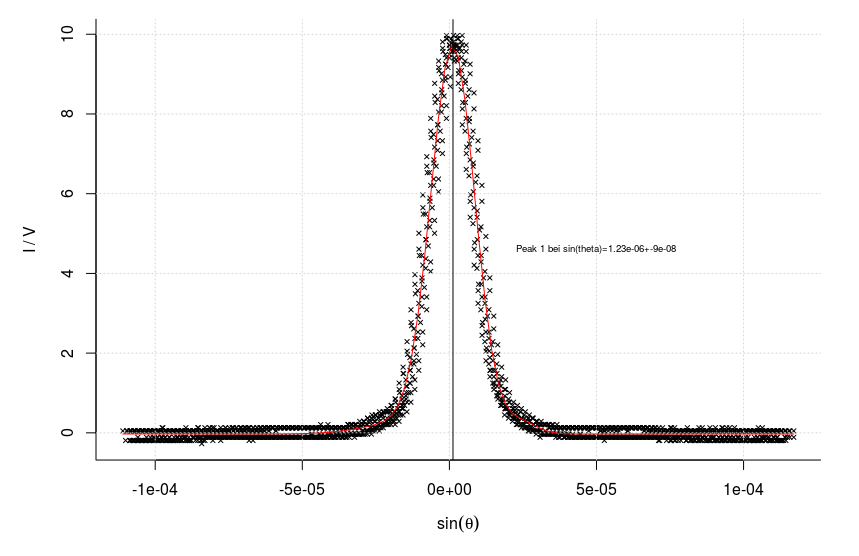
\includegraphics[width=0.49\textwidth]{figures/ultraschall1.png}\hskip 10 pt
	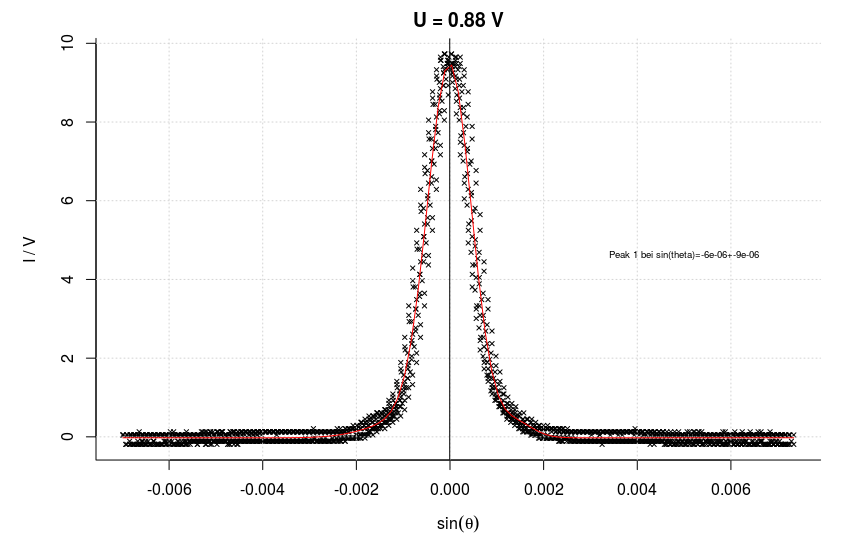
\includegraphics[width=0.49\textwidth]{figures/ultraschall2.png}\vskip 10 pt
	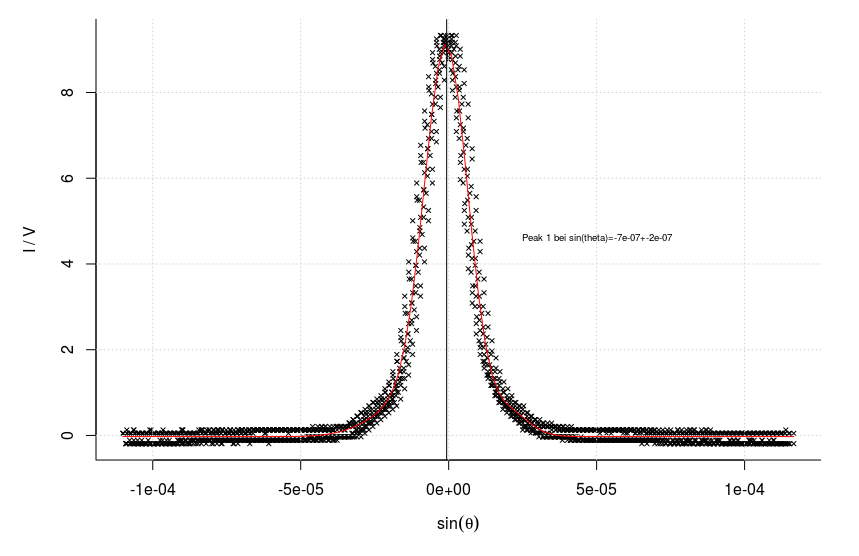
\includegraphics[width=0.49\textwidth]{figures/ultraschall3.png}\hskip 10 pt
	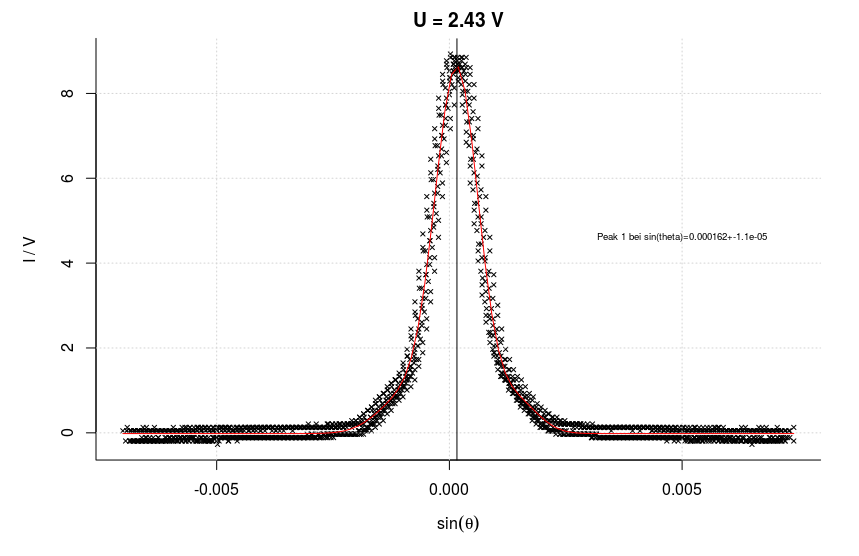
\includegraphics[width=0.49\textwidth]{figures/ultraschall4.png}\vskip 10 pt
	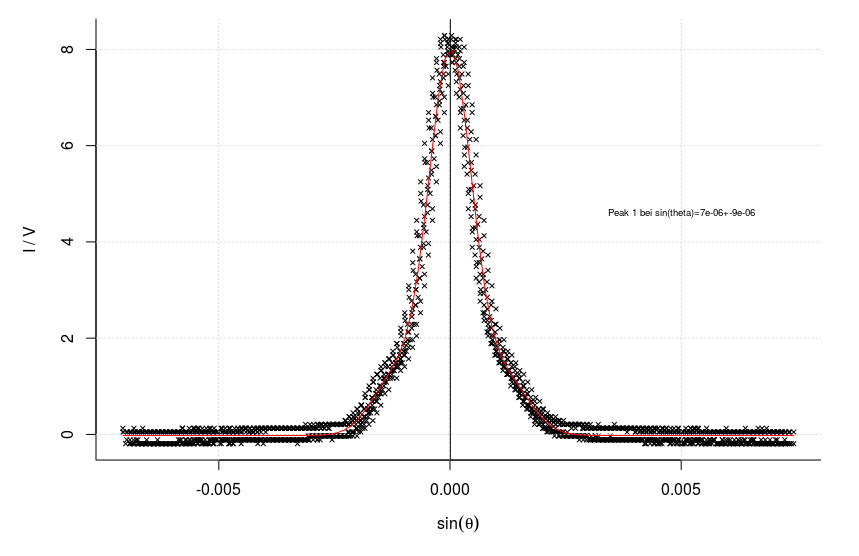
\includegraphics[width=0.49\textwidth]{figures/ultraschall5.png}\hskip 10 pt
	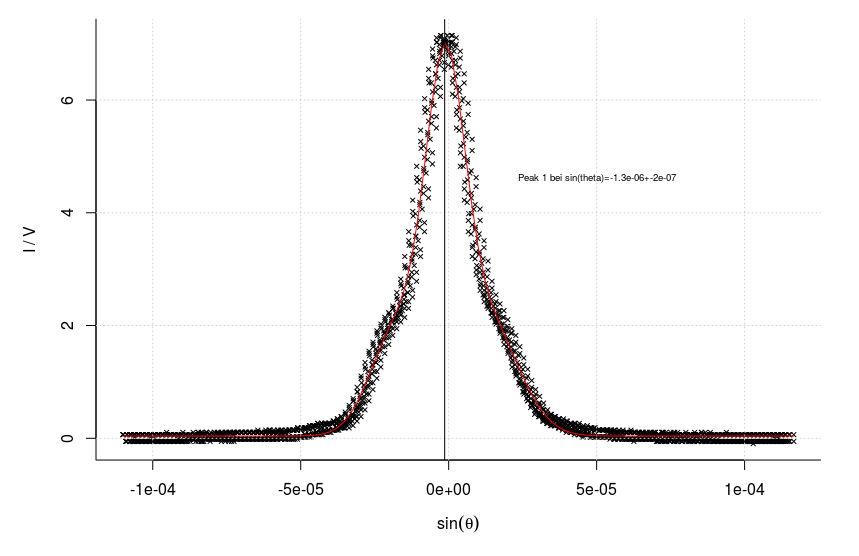
\includegraphics[width=0.49\textwidth]{figures/ultraschall6.png}\vskip 10 pt
	\captionof{figure}{Gaußfits an die Beugungsbilder der Spannungen 0 V bis 4.2 V}
\end{minipage}\newpage
\begin{minipage}[h!]{\textwidth}
	\centering
	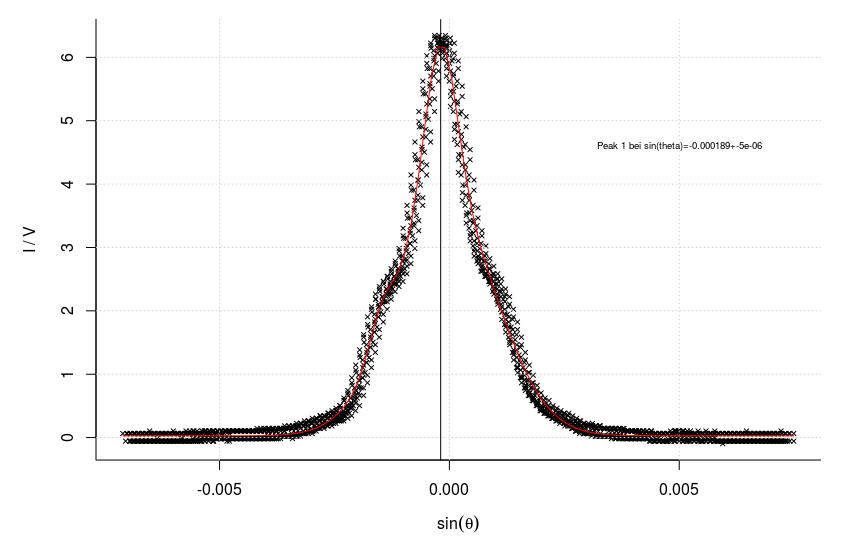
\includegraphics[width=0.49\textwidth]{figures/ultraschall7.png}\hskip 10 pt
	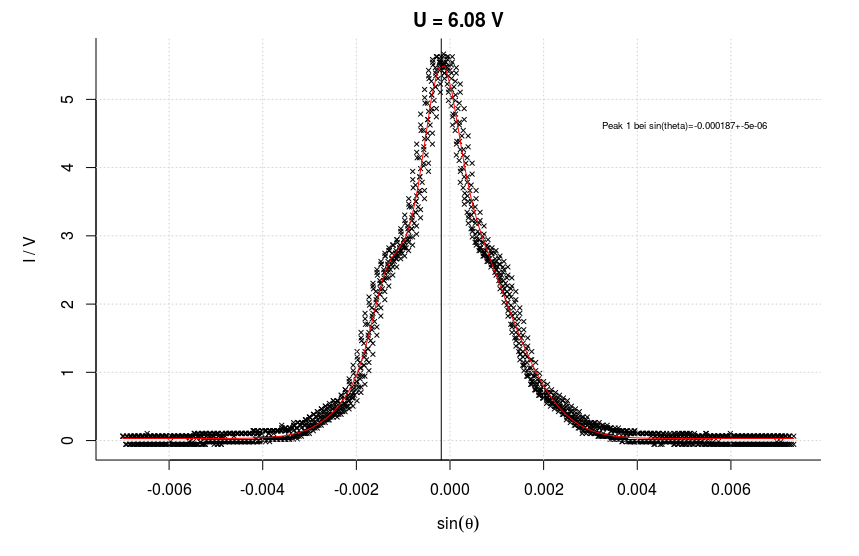
\includegraphics[width=0.49\textwidth]{figures/ultraschall8.png}\vskip 10 pt
	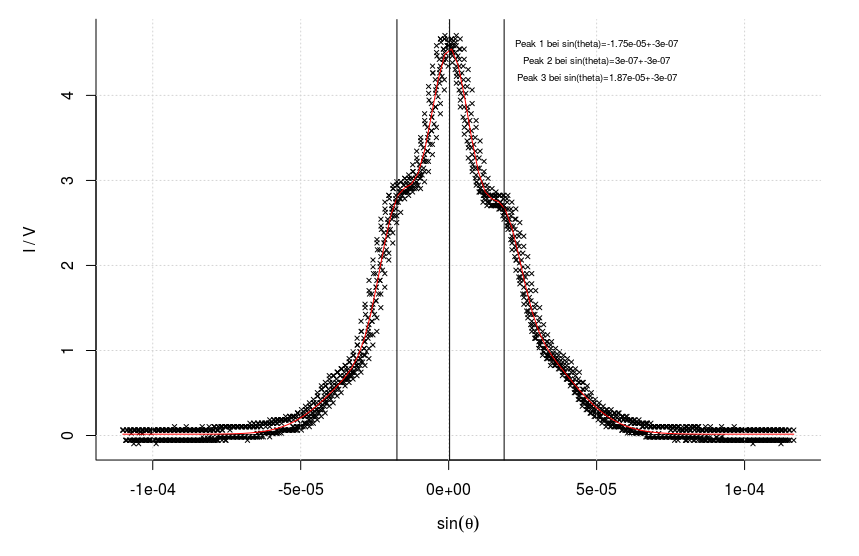
\includegraphics[width=0.49\textwidth]{figures/ultraschall9.png}\hskip 10 pt
	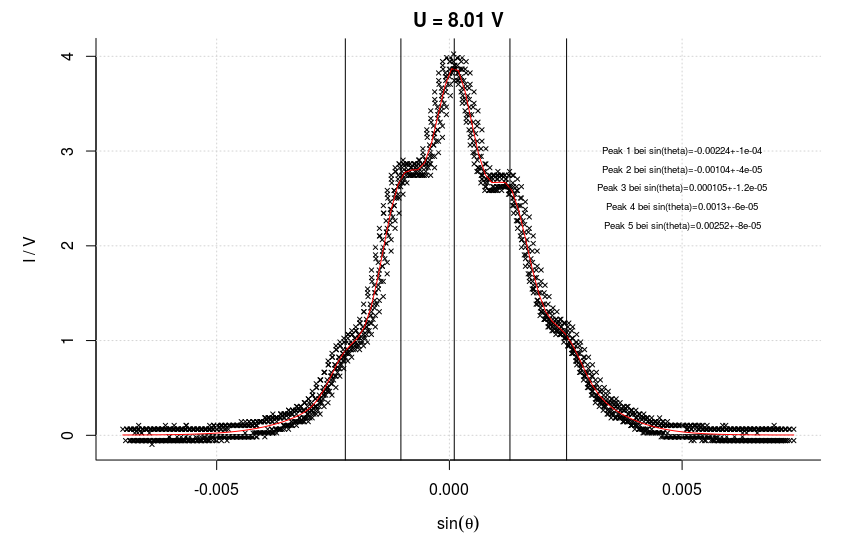
\includegraphics[width=0.49\textwidth]{figures/ultraschall10.png}\vskip 10 pt
	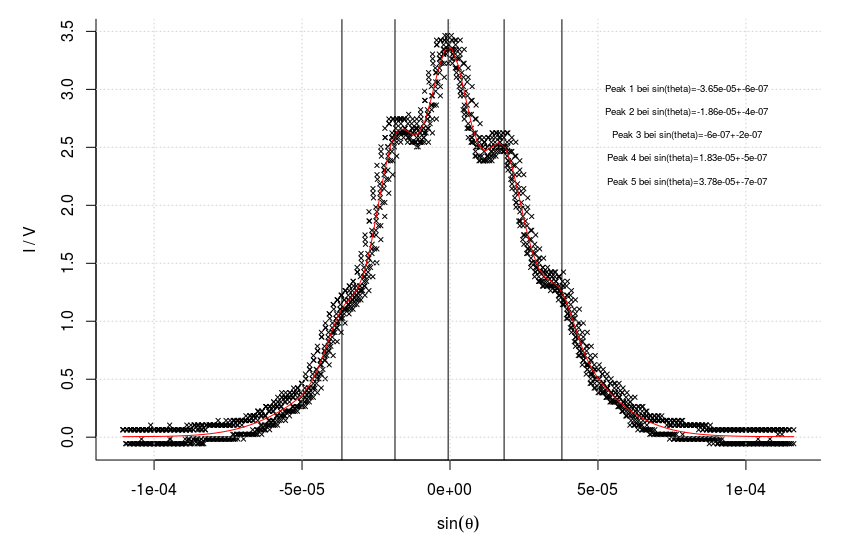
\includegraphics[width=0.49\textwidth]{figures/ultraschall11.png}\hskip 10 pt
	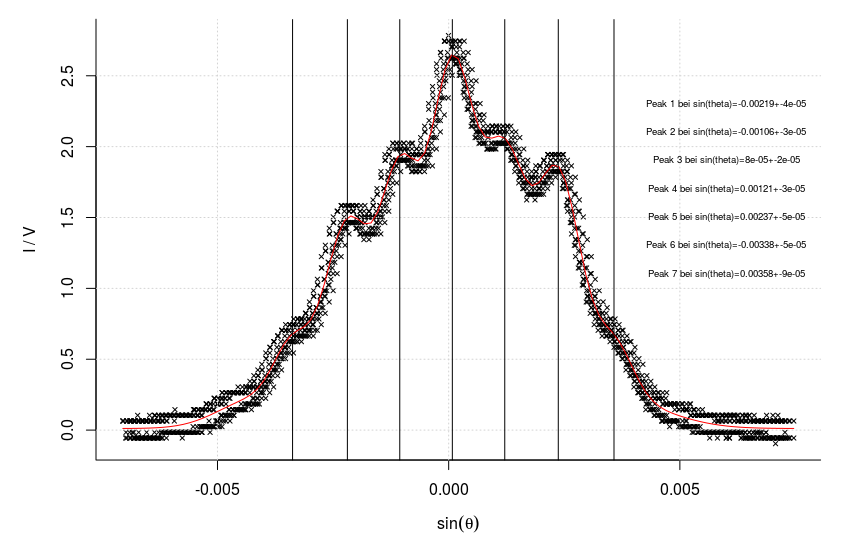
\includegraphics[width=0.49\textwidth]{figures/ultraschall12.png}\vskip 10 pt
	\captionof{figure}{Gaußfits an die Beugungsbilder der Spannungen 5.1 V bis 9.69 V}
\end{minipage}\newpage
\subsection{Laborheft\label{Laborheft}} 
\begin{minipage}{\textwidth}
\centering
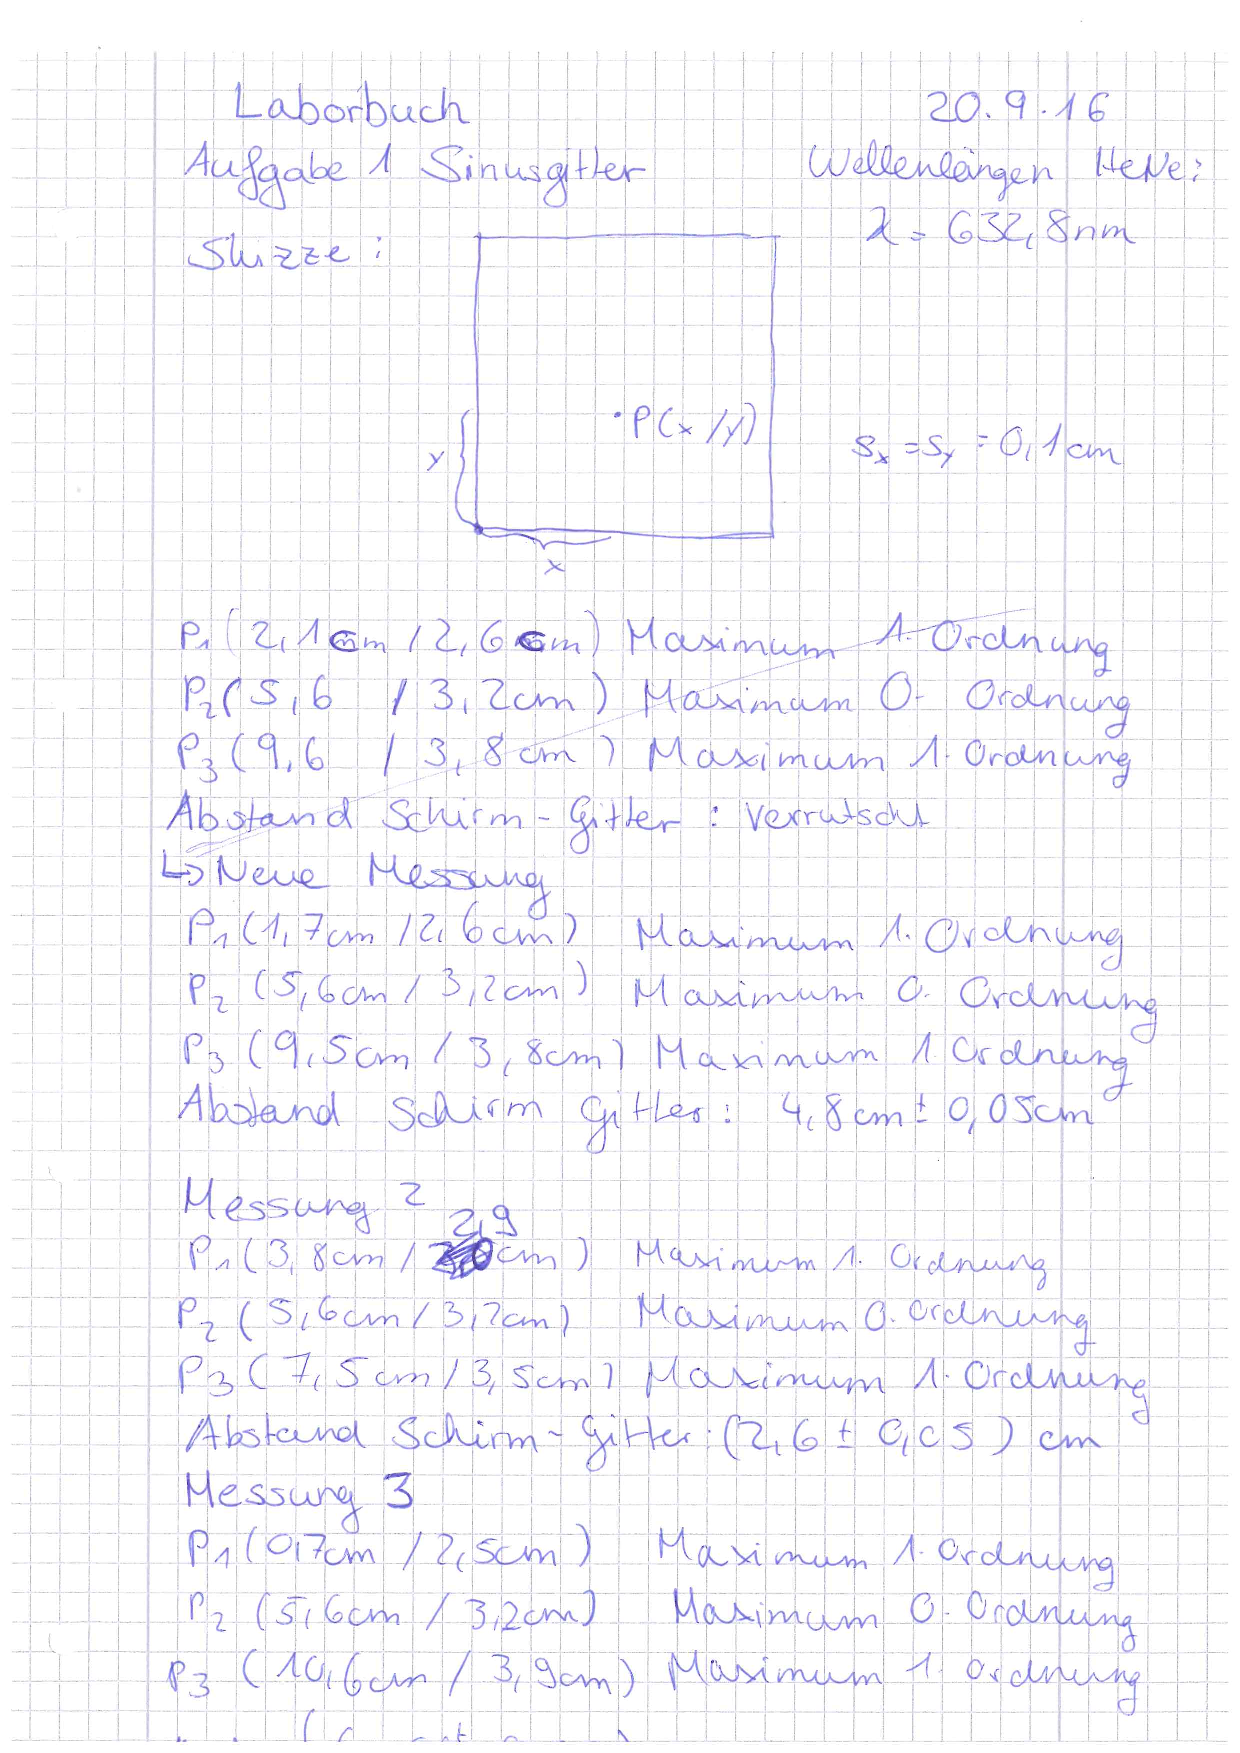
\includegraphics[width=0.9\textwidth]{figures/Laborbuch2.pdf}
\end{minipage}

\begin{minipage}{\textwidth}
\centering
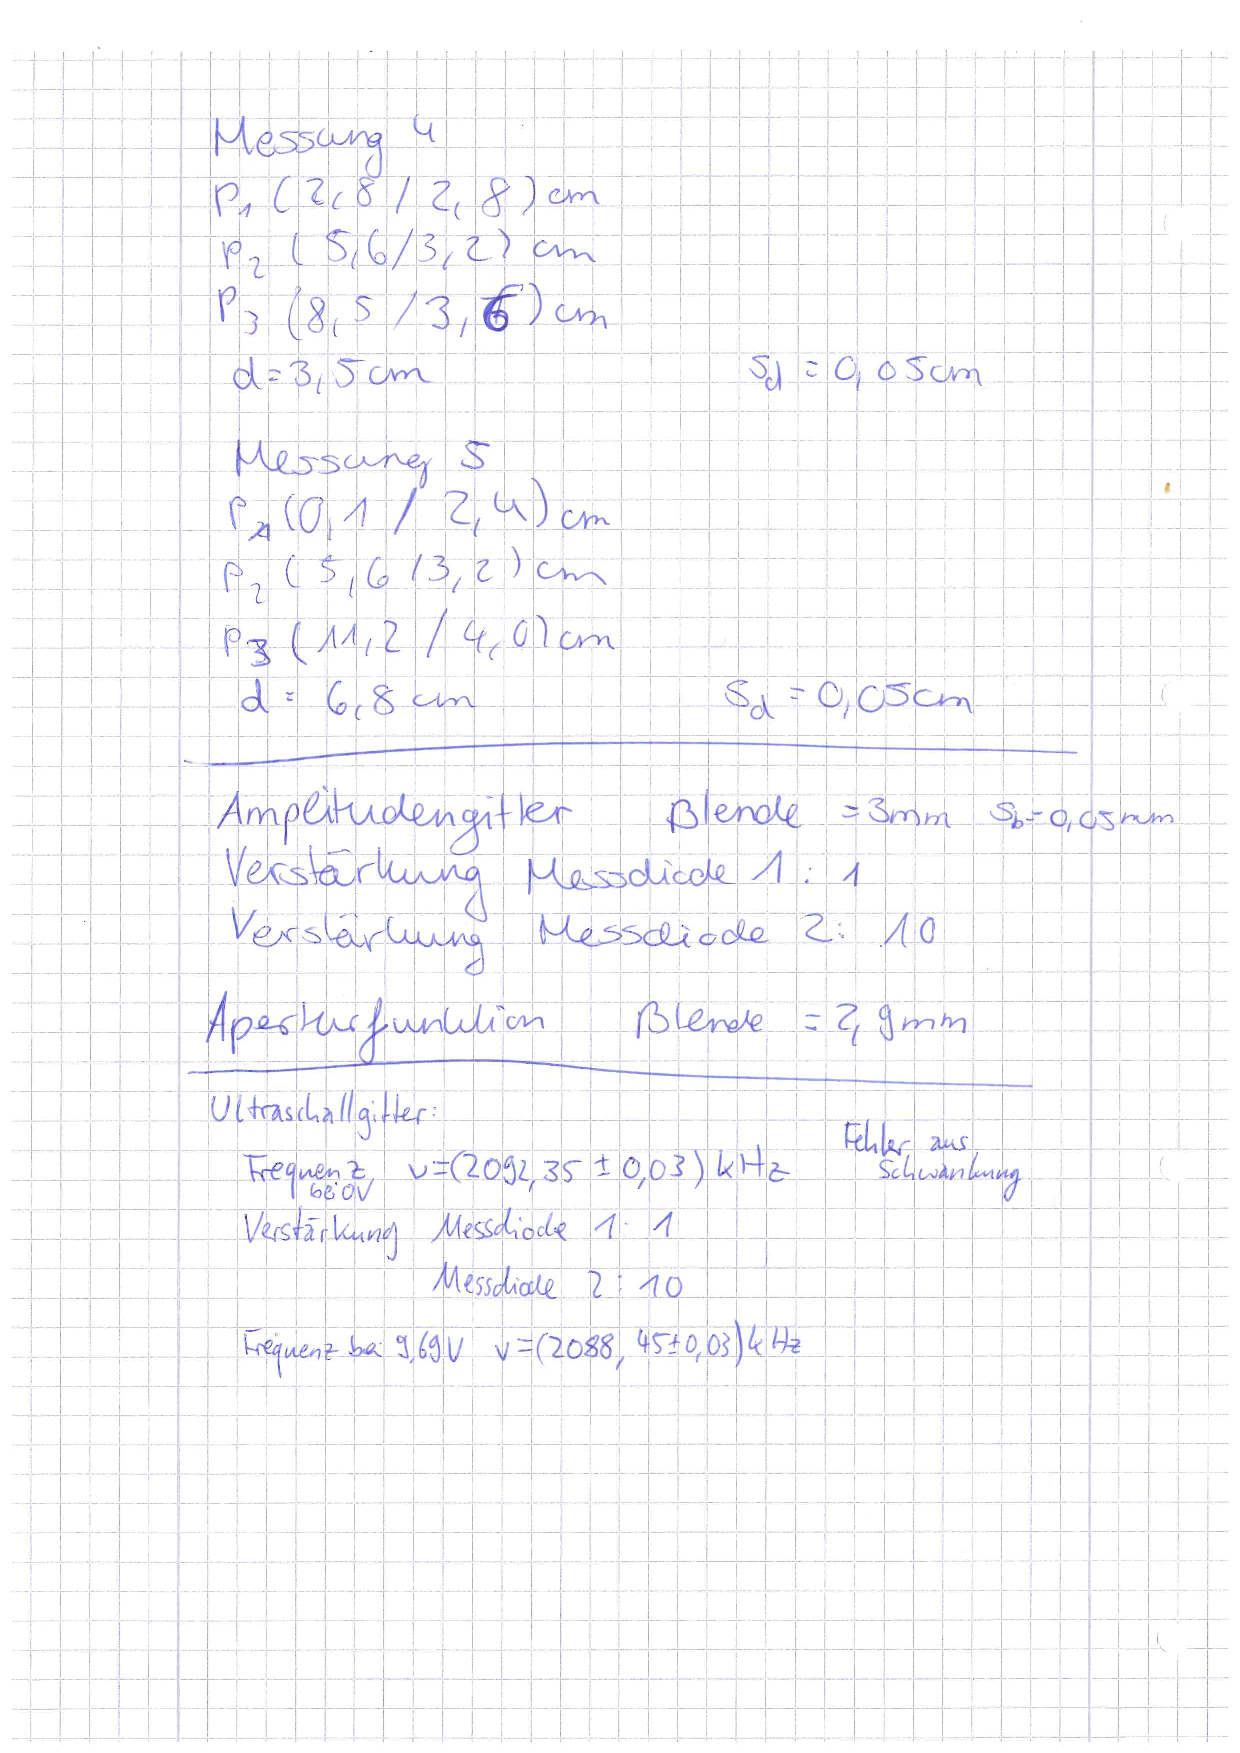
\includegraphics[width=0.9\textwidth]{figures/Laborbuch1.pdf}
\end{minipage}
\newpage
\listoffigures

%Literatur----------------------------------------------------------------------------------------------------------

%\cite{les}
\newpage
\thispagestyle{empty}
\begin{thebibliography}{9}

\bibitem{kirch}
  G. Kirchhoff,
  \emph{Zur Theorie der Lichtstrahlen},
  Annalen der Physik,
  Vol. 254,
  1882
\bibitem{good}
  Joseph W. Goodman,
  \emph{Introduction to Fourier Optics},
  Stanford University,
  2nd sedition,
  1996
\bibitem{rana}
  C.V. Raman, N.S. Nagendra Nath,
  \emph{Diffraction of Light by High Frequency Sound Waves: Part 1},
  Indian Institute of Science Bangalore,
  1935
\bibitem{anleitung}
  M. Köhli,
  \emph{Versuchsanleitung Fortgeschrittenen Praktikum: Ultraschall},
  Albert-Ludwigs-Universität Freiburg,
  2011
  
\bibitem{staat}
  Lutz Lefevre,
  \emph{Beugung am Amplitudengitter und Phasengitter},
  Albert-Ludwigs-Universität Freiburg,
  1977

\bibitem{Demtröder}
Wolfgang Demtröder
 \emph{Experimentalphysik 2: Elektrizität und Optik},
 Springer-Verlag,
 6. Auflage,
 2014
\end{thebibliography}

\end{document}